\documentclass[ngerman,a4paper]{texmf/tex/latex/mathscript/mathscript}
\usepackage{texmf/tex/latex/mathoperators/mathoperators}

\title{\textbf{Interpolation der \person{Runge}-Funktion und anderer Funktionen mit Octave}}

\begin{document}
\maketitle
	
\tableofcontents
\pagebreak
	
\section{Interpolation der \person{Runge}-Funktion}	
	\begin{align}
		f(x) &= \frac{1}{1+25x^2}\notag \\
		f' (x) &= -\frac{50x}{625x^4+50x^2+1}\notag
	\end{align}
	
	\subsection{Berechnung der Splines}\label{1.1}
	\subsubsection{Polynomsplines aus $\mathcal{S}_1^0(\Delta)$}
	
	Eine Polynomspline $s\in\mathcal{S}_1^0(\Delta)$ ist eine affin lineare Funktion, das heißt er hat die Form $s(x)=mx+n$ mit Anstieg $m$ und $y$-Achsenverschiebung $n$. 
	
	Die Interpolationsfunktion $g_N$, mit $N+1$ Stützstellen, besteht nun also aus Splines $s_i\in\mathcal{S}_1^0(\Delta)$, wobei für jeden Spline gilt:
	\begin{align}
		\text{Definitionsbereich: } & [x_i,x_{i+1}] \notag \\
		m_i =& \frac{f_{i+1}-f_i}{x_{i+1}-x_i}\notag \\
		n_i =& f_i \notag
	\end{align} 
	wobei $x_i$ die Stützstellen und $f_i$ die Stützwerte sind. Dabei läuft $i$ von $0$ bis $N-1$.
	
	Der Quelltext für Octave sieht dann so aus:
\begin{lstlisting}
runge = @(x) 1./(1+25*x.^2);
xreal = -1:0.01:1;

n = input('Anzahhl der Stuetzstellen - 1 := N: ');

%Schritweite h berechnen
h = 2/n
%Stuetzstellenvektor x berechnen
x = -1:h:1;

for i=1:n+1
 %Stutzwertevektor f berechnen
 f(i) = runge(x(i));
endfor

for i=1:n
 %Anstiege m_i berechnen
 m(i) = (f(i+1)-f(i))./(x(i+1)-x(i));
 %Achsenabschnitte n_i berechnen
 n(i) = f(i);
endfor

plot(x, f, "-;Interpol.;", xreal, runge(xreal), "-;Rungefkt.;")
\end{lstlisting}

	Das Interessante hierbei ist, dass die berechneten Werte in den Arrays \texttt{m} und \texttt{n} gar nicht für die Interpolation gebraucht werden - die Funktion \texttt{plot} interpoliert automatisch linear, wenn man ihr die Stützstellen und -werte übergibt.
	
	\begin{figure}[h]
		\centering
		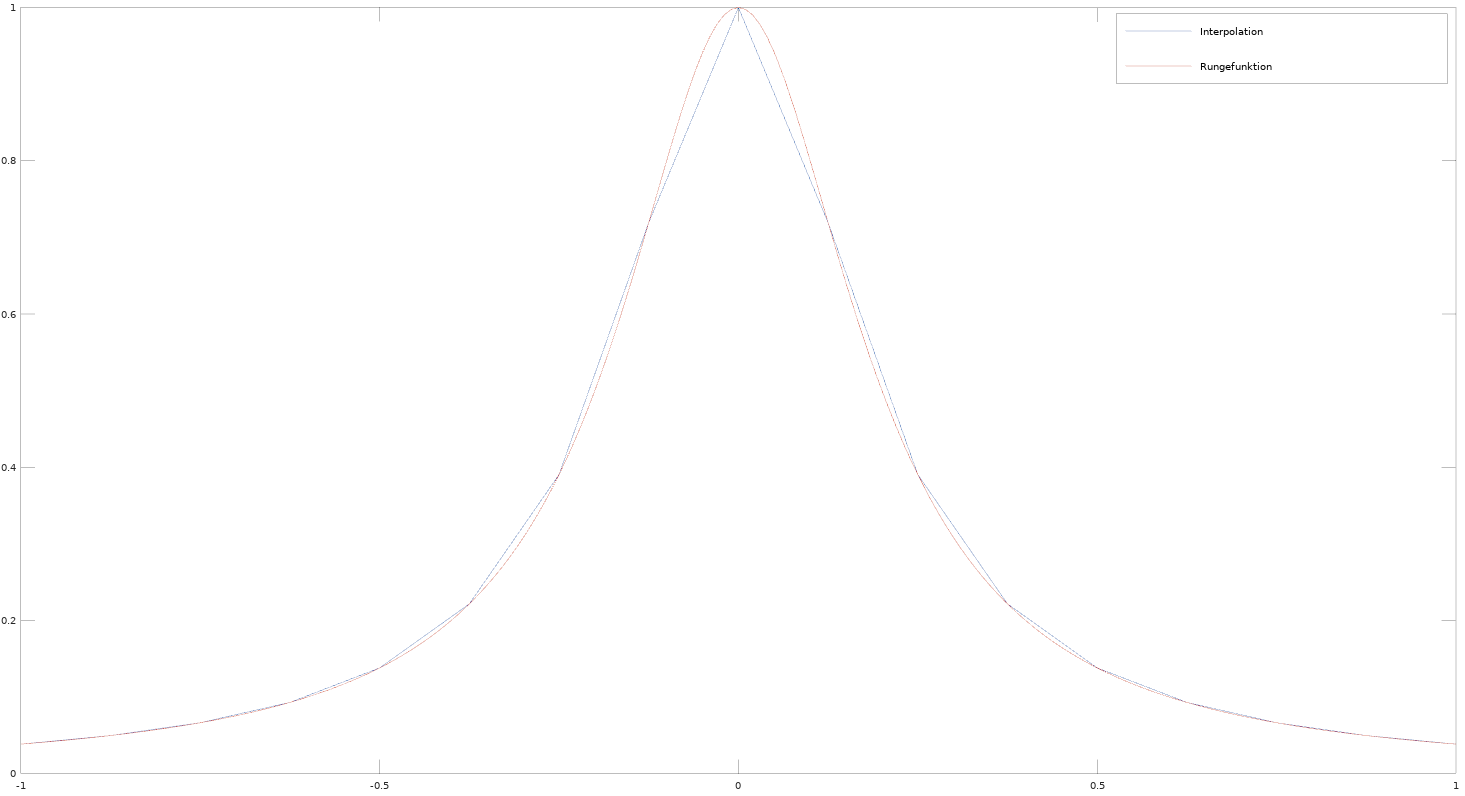
\includegraphics[width=0.9\textwidth]{images/Runge_lineare_Interpolation.png}
		\caption{lineare Splineinterpolation mit $N=16$}
	\end{figure}

	\begin{figure}[h]
		\centering
		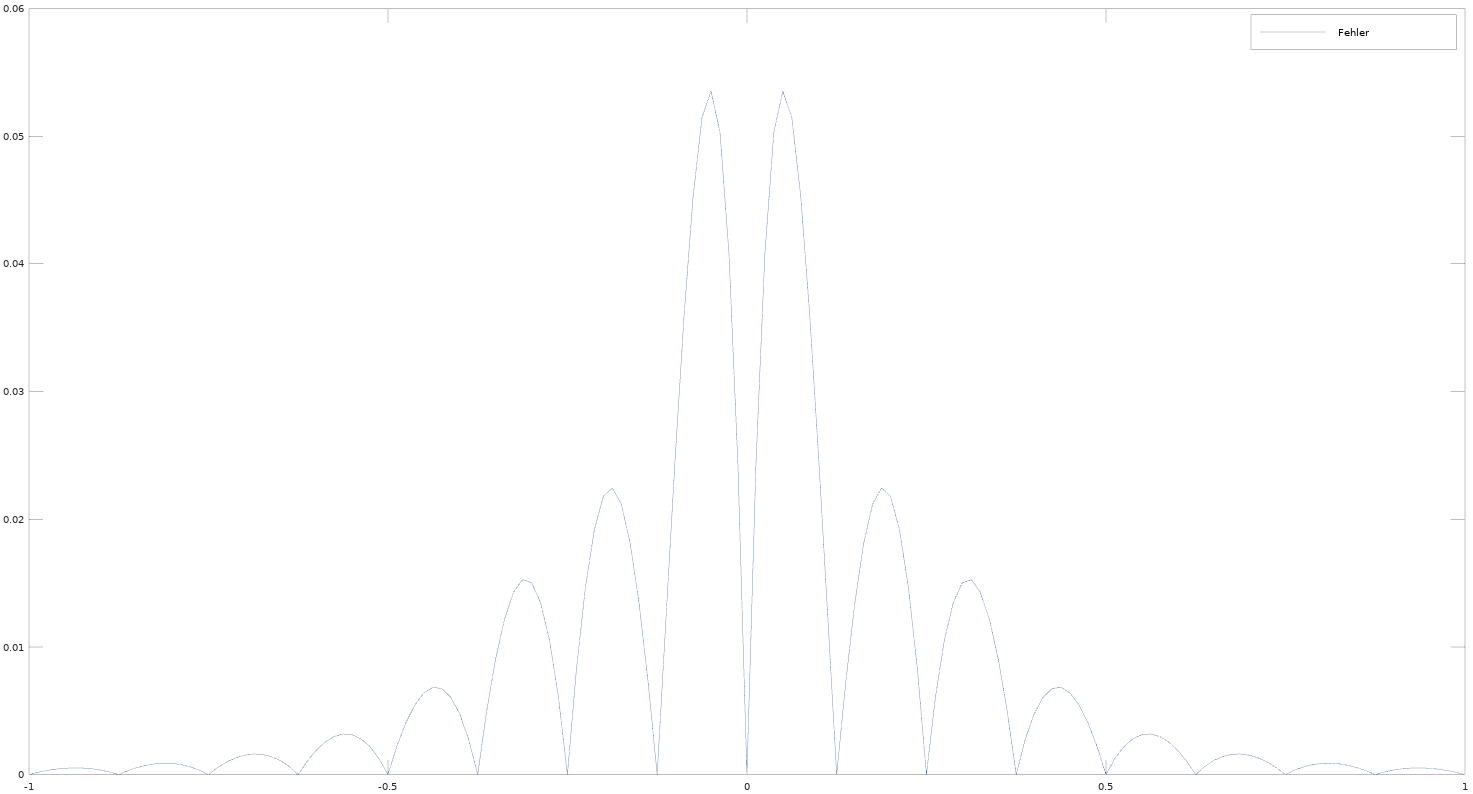
\includegraphics[width=0.9\textwidth]{images/Runge_lineare_Interpolation_Fehler.png}
		\caption{Fehler bei linearer Splineinterpolation mit $N=16$}
	\end{figure}
	
	\subsubsection{Polynomsplines aus $\mathcal{S}_3^1(\Delta)$}
	
	Da die Interpolationssplines Polynome dritten Grades und einmal stetig differenzierbar sein sollen, nehmen wird aus der Vorlesung den Ansatz (1.7):
	\begin{align}
		s_k(x) = a_k(x-x_k)^3 + b_k(x-x_k)^2 + c_k(x-x_k) + d_k\notag
	\end{align}
	mit $x\in[x_k,x_{k+1}]$. Die Vorfaktoren $a_k$, $b_k$, $c_k$ und $d_k$ ergeben sich aus (1.9) und (1.10) in der Vorlesung.
	\begin{align}
		d_k &= f_k \notag \\
		c_k &= m_k = s'(x_k) = f'(x_k) \notag \\
		\begin{pmatrix}
			h_k^3 & h_k^2 \\ 3h_k^2 & 2h_k
		\end{pmatrix}\begin{pmatrix}
			a_k \\ b_k
		\end{pmatrix} &= \begin{pmatrix}
			f_{k+1} - f_k - m_kh_k \\ m_{k+1} - m_k
		\end{pmatrix}\notag
	\end{align}
	wobei $h_k$ mit $\frac{2}{N}$ gegeben war. Der Quelltext sieht dann folgendermaßen aus:
	\begin{lstlisting}
runge = @(x) 1./(1+25*x.^2);
runge_abl = @(x) (-50*x)/(1+25*x^2)^2;

N = input('Anzahl der Stuetzstellen -1 :=N : ')

%Abstand Stuetzstellen h
h = 2/N;

%Stuetzstellen x
x = -1:h:1;

for i = 1:N+1
 %Stuetzwerte f
 f(i) = runge(x(i));
 %Ableitungen
 m(i) = runge_abl(x(i));
endfor

%Berechnung a_k, b_k nach 1.10
H = [h^3 , h^2 ; 3*h^2 , 2*h];
for i = 1:N
 r = H\[f(i+1)-f(i)-m(i)*h ; m(i+1)-m(i)];
 a(i) = r(1);
 b(i) = r(2);
 %c(i) = m(i)
 %d(i) = f(i)
endfor

%Interpolierende und Runge plotten auf Zerlegung M
M = 10 * N;
h_fein = 2/M;
x_fein = -1:h_fein:1;
k = 1;
for i=1:N
 %in jedem dieser Durchlaeufe ist der Spline-Abschnitt der Selbe
 for j=1:10
  s(k) = a(i)*(x_fein(k)-x(i))^3 +b(i)*(x_fein(k)-x(i))^2 +...
  m(i)*(x_fein(k)-x(i))+f(i);
  k = k + 1;
 endfor
endfor

s(k) = f(N+1);

figure(1);
plot(x_fein, runge(x_fein), "-;Funktion;", x_fein, ...
s,"-;Interpolation;")
	\end{lstlisting}
	
	\begin{figure}[h]
		\centering
		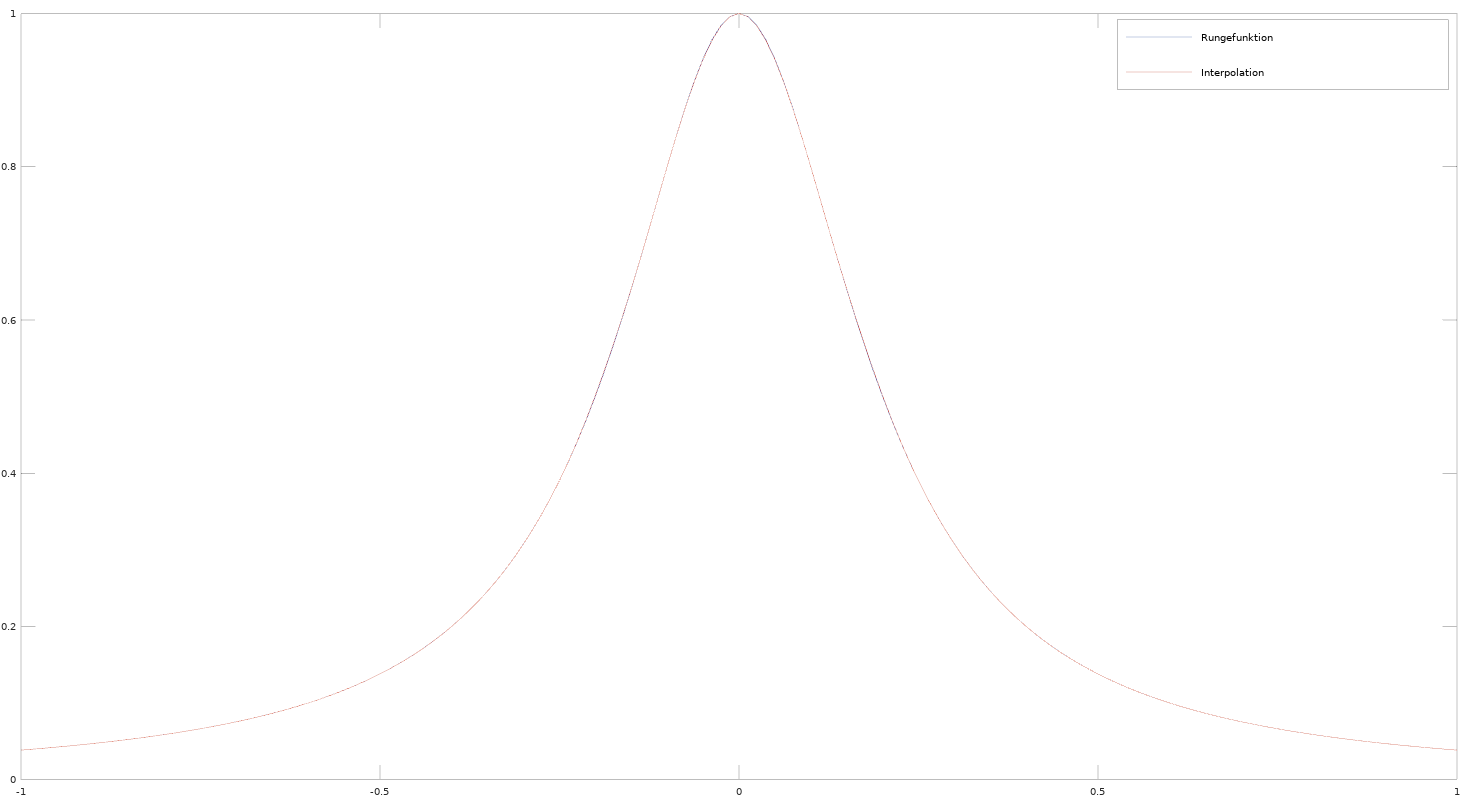
\includegraphics[width=0.9\textwidth]{images/Runge_kubische_Interpolation.png}
		\caption{kubische Splineinterpolation mit $N=16$}
	\end{figure}
	\pagebreak
	
	\begin{figure}[h]
		\centering
		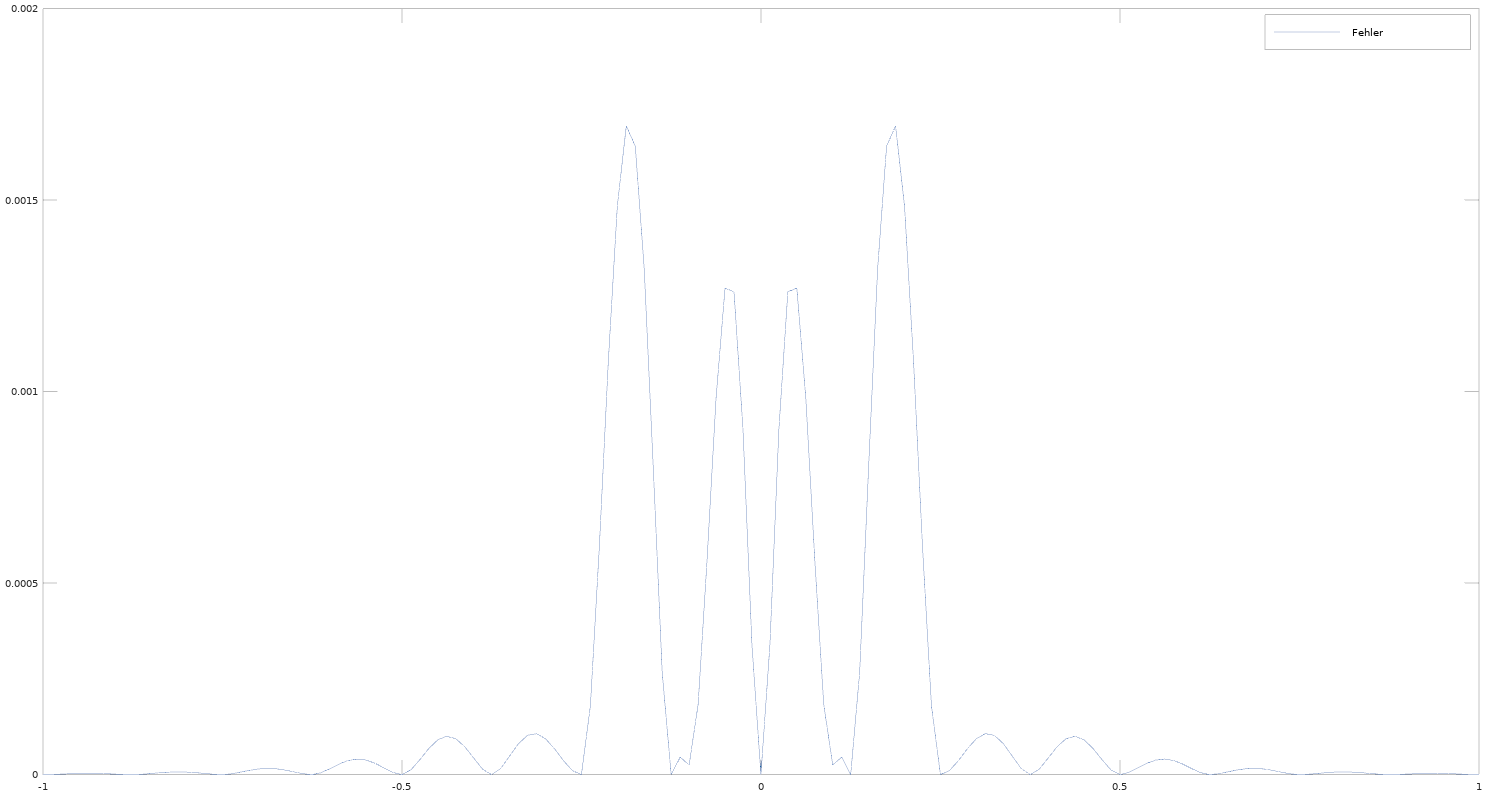
\includegraphics[width=0.9\textwidth]{images/Runge_kubische_Interpolation_Fehler.png}
		\caption{Fehler bei kubischer Splineinterpolation mit $N=16$}
	\end{figure}
	
	\subsection{Fehlerbetrachtung}
	
	Da $\Delta_M$ zehnmal so fein wie $\Delta_N$ ist, bedeutet das, dass man für jeden Spline den Fehler in 10 Punkten in seinem Definitionsbereich berechnet.
	
	Bei linearer Interpolation kann man also deswegen den Fehler nach folgendem Muster ausrechnen:
	\begin{align}
		\text{Fehler} = \vert f(x) - (n + \text{Abstand zur nächsten Stützstelle}\cdot m) \vert \notag
	\end{align}
	wobei $n$ und $m$ zum jeweiligen Spline gehören und $x$ die Werte in $\Delta_M$ durchläuft. Da die Fehlerfunktion laut Aufgabenstellung an den Stützstellen der Zerlegung $\Delta_M$ zu berechnen ist, lässt sich der nachfolgende Code auch für die Abschätzung des Fehlers (der auch an den Stützstellen von $\Delta_M$ gesucht ist) wiederverwenden. Der Quelltext dazu sieht folgendermaßen aus:
\begin{lstlisting}
M = 10 * N
h_neu = 2/M
x_Fehler = -1:h_neu:1;

k = 1;
for i=1:N
 %in jedem dieser Durchlauufe ist der Spline-Abschnitt der Selbe
 for j=1:10
  y_Fehler(k) = abs(runge(x_Fehler(k)) - ...
   (n(i) + abs(abs(x_Fehler(k)) - abs(x(i))) * m(i)));
  k = k + 1;
 endfor
endfor

%Fehler an letzter Stuetzstelle ist 0
y_Fehler(k) = 0;

plot(x_Fehler, y_Fehler, "-; Fehler;")

% maximaler Fehler E
E = max(y_Fehler)
\end{lstlisting}

Für die Fehlerberechnung bei kubischer Interpolation haben wir wieder den Ansatz $s_k(x) = a_k(x-x_k)^3 + b_k(x-x_k)^2 + c_k(x-x_k) + d_k$ verwendet.
\begin{lstlisting}
%Fehlerfunktion

k = 1;
 for i=1:N
 %in jedem dieser Durchlaeufe ist der Spline-Abschnitt der Selbe
 for j=1:10
  y_Fehler(k) = abs(runge(x_fein(k)) - ...
  (a(i)*(x_fein(k)-x(i))^3 +b(i)*(x_fein(k)-x(i))^2 +...
  m(i)*(x_fein(k)-x(i))+f(i)));
  k = k + 1;
 endfor
endfor

%Fehler an letzter Stuetzstelle ist 0
y_Fehler(k) = 0;

figure(2);
plot(x_fein, y_Fehler, "-; Fehler;")

%Maximaler Fehler
E = max(y_Fehler);
\end{lstlisting}
	
	\subsection{Diskussion der Ergebnisse}
	
	Der maximale Fehler $E(h_N)$ für $N=N_k=4\cdot 2^k$ mit $k=0,...,4$ beträgt:
	\begin{center}
		\begin{tabular}{ll|l|l}
			$k$ & $N_k$ & $E(h_{N_k})$ $\mathcal{S}_1^0$ & $E(h_{N_k})$ $\mathcal{S}_3^1$ \\
			\hline
			0 & 4 & 0.17872 & 0.21938 \\
			\hline
			1 & 8 & 0.063128 & 0.035509 \\
			\hline 
			2 & 16 & 0.053536  & 0.0016935\\
			\hline 
			3 & 32 & 0.020652  & 0.00038860\\
			\hline 
			4 & 64 & 0.0058496 & 0.000033560\\
		\end{tabular}
	\end{center} 

Man sieht also, dass bei großen $N$ der Fehler sehr klein wird und die kubische Splineinterpolation besser als die lineare Interpolation ist.

Die exponentielle Konvergenzordnung ist
\begin{center}
	\begin{tabular}{ll|l|l}
		$k$ & $N_k$ & $EOC(h_{N_k},h_{N_{k+1}})$ $\mathcal{S}_1^0$ & $EOC(h_{N_k},h_{N_{k+1}})$ $\mathcal{S}_3^1$ \\
		\hline
		0 & 4 & 1.5013 & 2.6272\\
		\hline
		1 & 8 & 0.2378 & 4.3901\\
		\hline
		2 & 16 & 1.3742 & 2.1237\\
		\hline
		3 & 32 & 1.8199 & 3.5334\\
		\hline
		4 & 64 & 1.9541 & 3.8869\\
		\hline
		5 & 128 & 1.9885 & 3.9719\\
		\hline
		6 & 256 & 1.9971 & 3.9930\\
		\hline
		7 & 512 & 1.9992 & 3.9982\\
		\hline
		8 & 1024 & 1.9998 & 3.9996\\
		\hline
		9 & 2048 & 2.0000 & 3.9999\\
		\hline
		10 & 4096 & 2.0000 & 4.0000\\
		\hline
	\end{tabular}
\end{center}

Mit $k=11$, $N=8192$ ist $h_{N_k}= \frac{2}{8192}$. Da EOC ein Maß für die Konvergenzgeschwindigkeit ist, bedeutet das, dass die kubische Spline-Interpolation doppelt so schnell gegen die \person{Runge}-Funktion konvergiert wie die lineare Interpolation.

\section{Interpolation der anderen Funktion}
	\begin{align}
		f(x) &= \left( 1+\cos\left(\frac{3}{2}\pi x \right) \right)^{\sfrac{2}{3}}\notag \\
		f'(x) &=-\frac{\pi\sin\left(\frac{3}{2}\pi x\right)}{\sqrt[3]{1+\cos\left(\frac{3}{2}\pi x \right)}}\notag
	\end{align}
	
	\subsection{Berechnung der Splines}
	Für Rechenvorschrift siehe \ref{1.1}
	
	\begin{figure}[h]
		\centering
		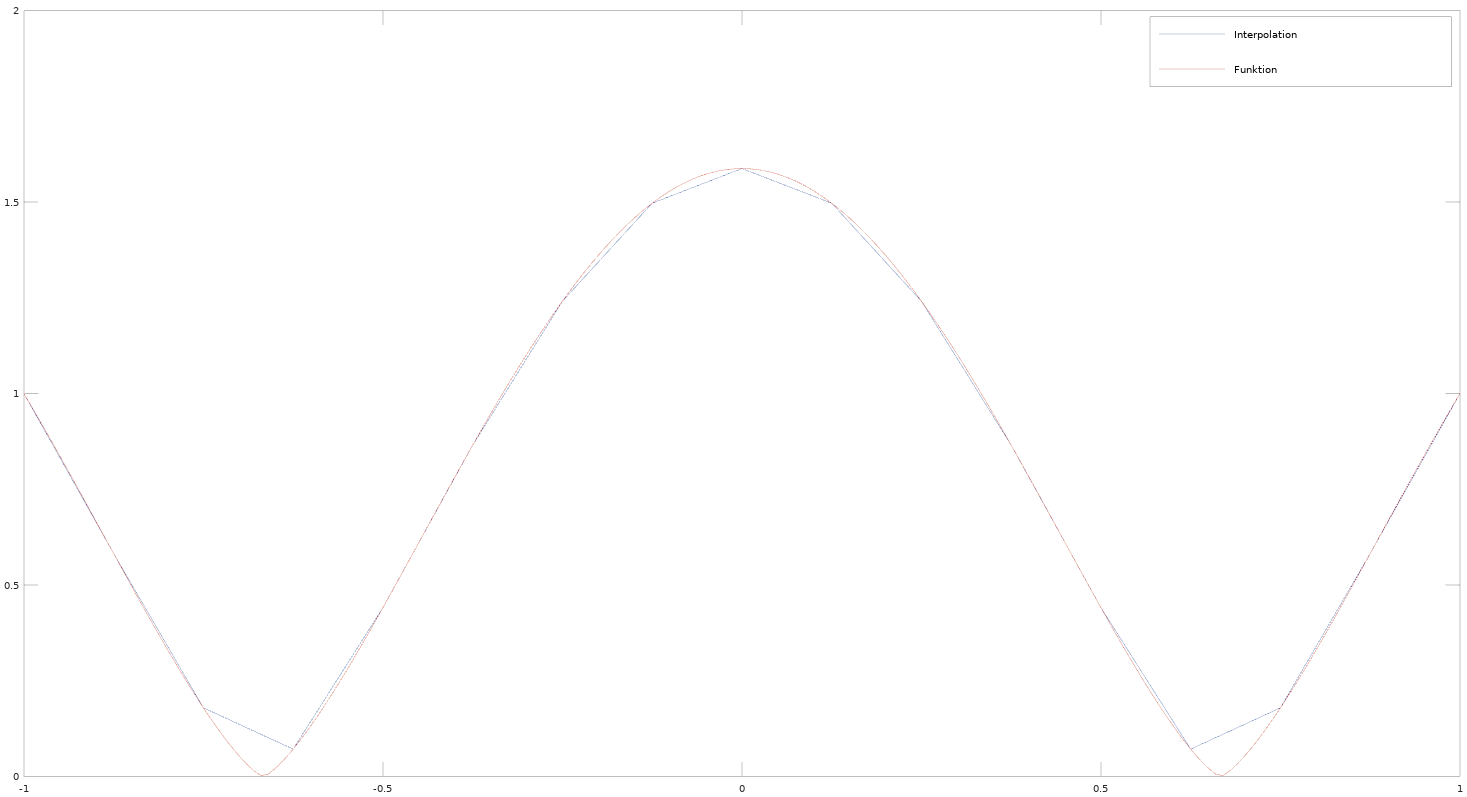
\includegraphics[width=0.9\textwidth]{images/f_lineare_Interpolation.png}
		\caption{lineare Splineinterpolation mit $N=16$}
	\end{figure}
	
	\begin{figure}[h]
		\centering
		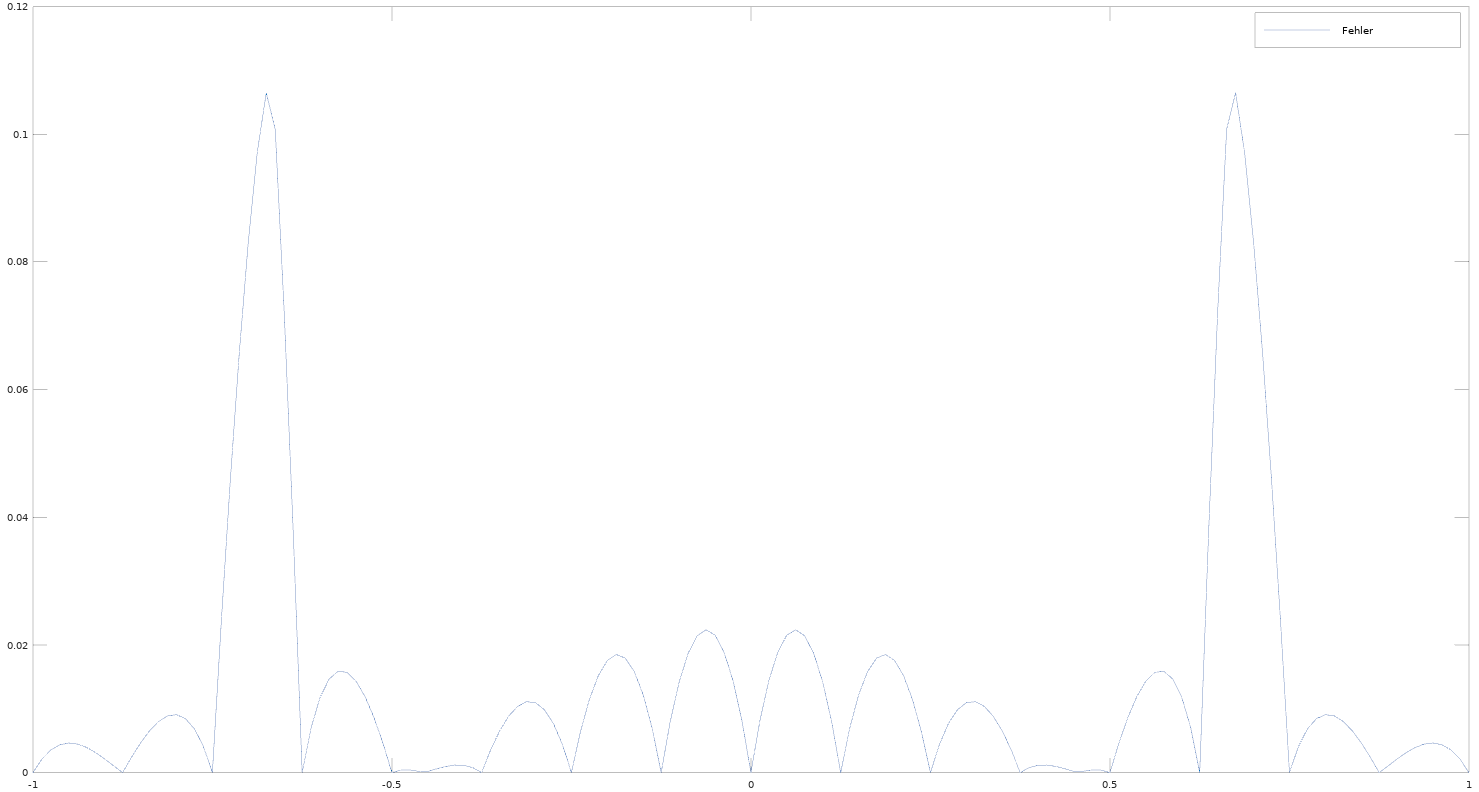
\includegraphics[width=0.9\textwidth]{images/f_lineare_Interpolation_Fehler.png}
		\caption{Fehler bei linearer Splineinterpolation mit $N=16$}
	\end{figure}

	\begin{figure}[h]
		\centering
		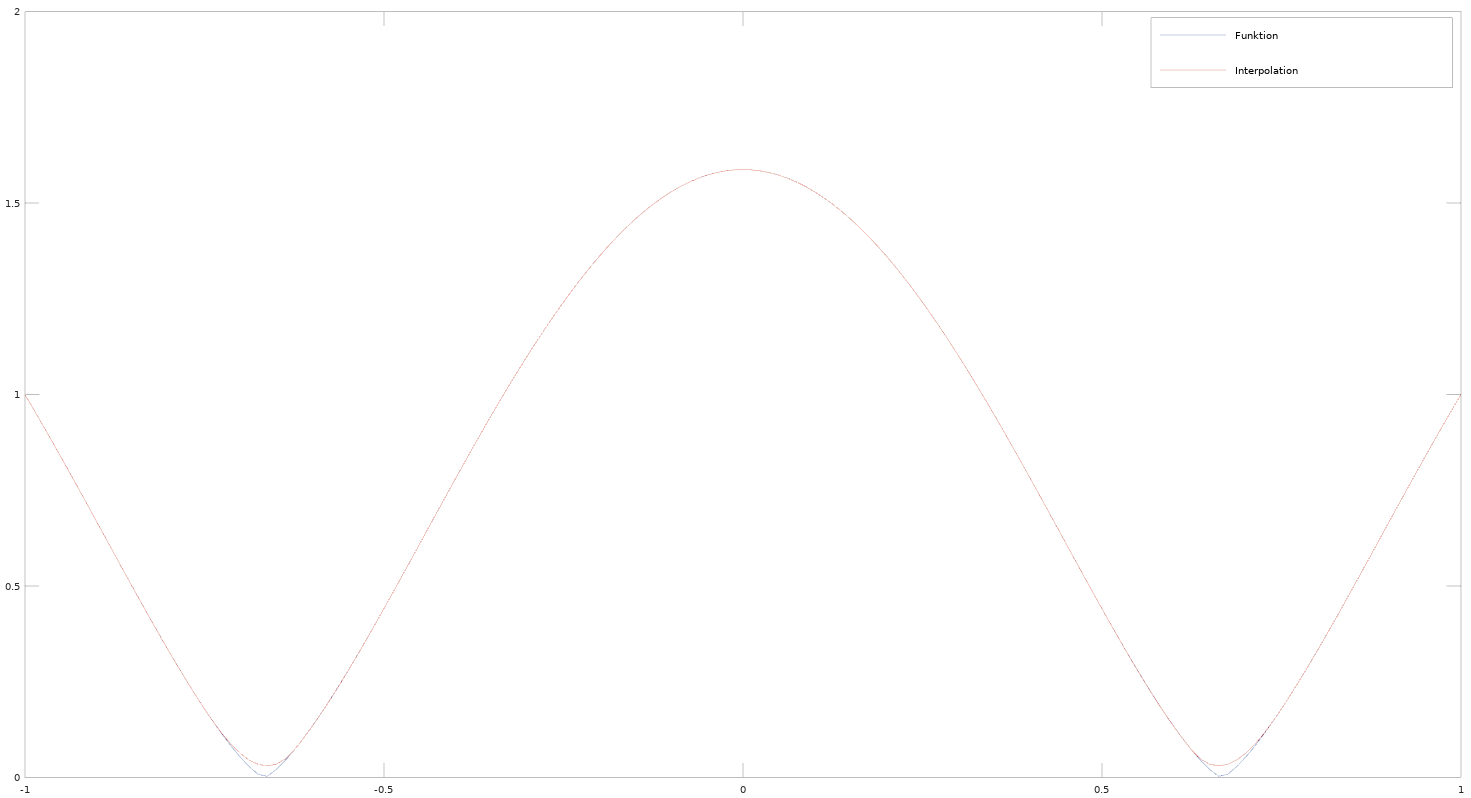
\includegraphics[width=0.9\textwidth]{images/f_kubische_Interpolation.png}
		\caption{kubische Splineinterpolation mit $N=16$}
	\end{figure}
	\pagebreak
	
	\begin{figure}[h]
		\centering
		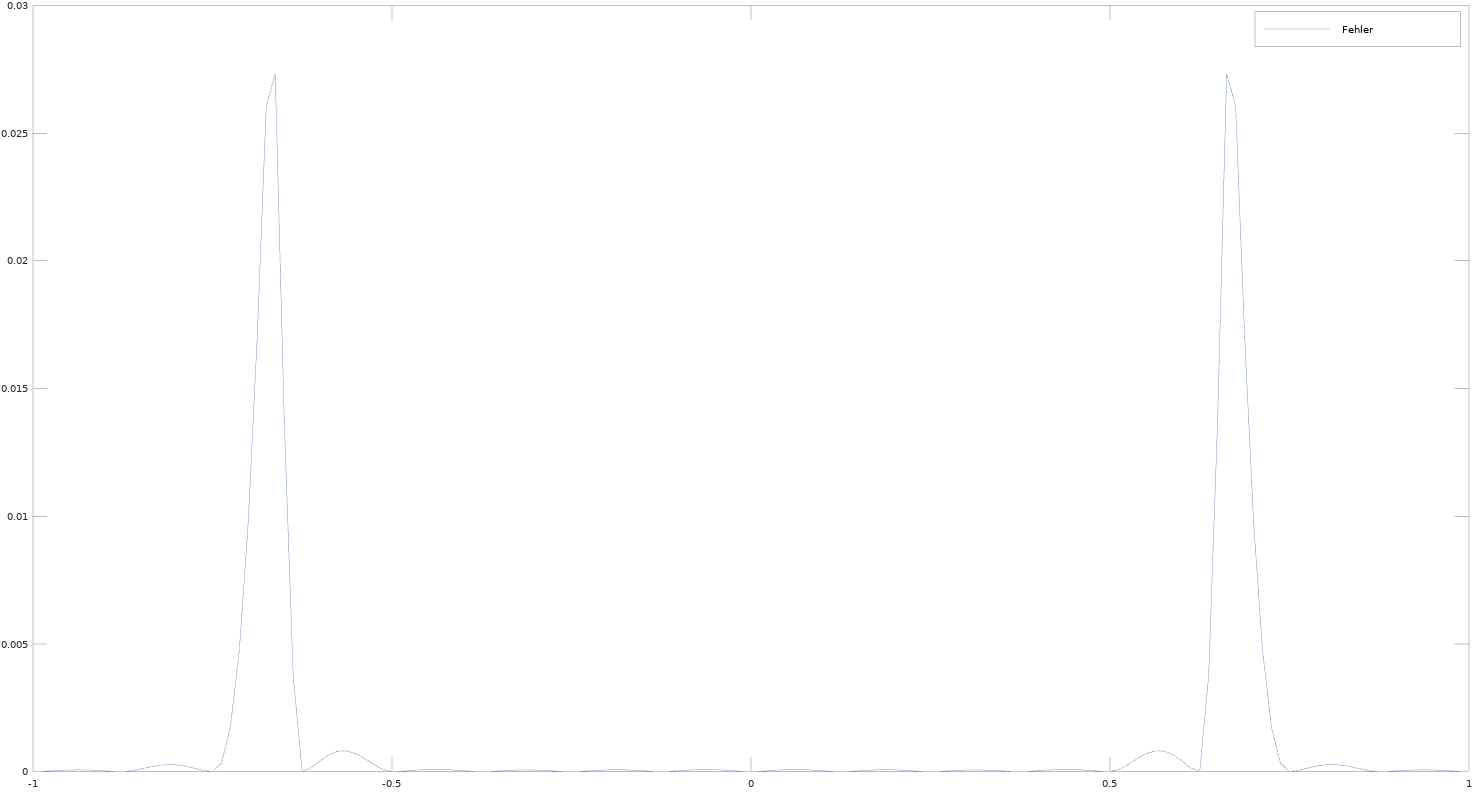
\includegraphics[width=0.9\textwidth]{images/f_kubische_Interpolation_Fehler.png}
		\caption{Fehler bei kubischer Splineinterpolation mit $N=16$}
	\end{figure}
	
	\subsection{Diskussion der Ergebnisse}
	
	Der maximale Fehler beträgt
	\begin{center}
		\begin{tabular}{ll|l|l}
			$k$ & $N_k$ & $E(h_{N_k})$ $\mathcal{S}_1^0$ & $E(h_{N_k})$ $\mathcal{S}_3^1$ \\
			\hline
			0 & 4 & 0.61130 & 0.19577 \\
			\hline
			1 & 8 & 0.26300 & 0.070736 \\
			\hline 
			2 & 16 & 0.10648 & 0.027316 \\
			\hline 
			3 & 32 & 0.042468 & 0.010764 \\
			\hline 
			4 & 64 & 0.016874 & 0.0042640 \\
		\end{tabular}
	\end{center} 

	Die exponentielle Konvergenzordnung ist
	\begin{center}
		\begin{tabular}{ll|l|l}
			$k$ & $N_k$ & $EOC(h_{N_k},h_{N_{k+1}})$ $\mathcal{S}_1^0$ & $EOC(h_{N_k},h_{N_{k+1}})$ $\mathcal{S}_3^1$ \\
			\hline
			0 & 4 & 1.2168 & 1.4686  \\
			\hline
			1 & 8 & 1.3045 & 1.3727\\
			\hline
			2 & 16 & 1.3261 & 1.3436 \\
			\hline
			3 & 32 & 1.3316 & 1.3359 \\
			\hline
			4 & 64 & 1.3328 & 1.3340 \\
			\hline
			5 & 128 & 1.3332 & 1.3335 \\
			\hline
			6 & 256 & 1.3332 & 1.3334 \\
			\hline
			7 & 512 & 1.3333 & 1.3333 \\
			\hline
			8 & 1024 & 1.3333 & 1.3333 \\
			\hline
			9 & 2048 & 1.3333 & 1.3333 \\
			\hline
			10 & 4096 & 1.3333 & 1.3333 \\
			\hline
		\end{tabular}
	\end{center}
	
	Mit $k=11$, $N=8192$ ist $h_{N_k}= \frac{2}{8192}$. Wenn EOC ein Maß für die Konvergenzgeschwindigkeit ist, dann konvergieren beide Ansätze - lineare und kubische Splineinterpolation - gleich schnell gegen diese Funktion.
	
	Offensichtlich ist diese Funktion nicht so gut für eine Splineinterpolation geeignet wie die \person{Runge}-Funktion, weil die maximalen Fehler größer sind und die EOC kleiner ist.

\end{document}
